\documentclass[runningheads,a4paper]{llncs}

\usepackage{amssymb} \setcounter{tocdepth}{3} \usepackage{graphicx}

\usepackage{url} \urldef{\mailsa}\path|{alfred.hofmann, ursula.barth,
  ingrid.haas, frank.holzwarth,| \urldef{\mailsb}\path|anna.kramer,
  leonie.kunz, christine.reiss, nicole.sator,|
  \urldef{\mailsc}\path|erika.siebert-cole, peter.strasser,
  lncs}@springer.com|
\newcommand{\keywords}[1]{\par\addvspace\baselineskip
  \noindent\keywordname\enspace\ignorespaces#1}

% added by Wei Liu
\usepackage{lwdefs}


\begin{document}

\mainmatter % start of an individual contribution


\title{Spatial Regularization of Functional Connectivity Using
  High-Dimensional Markov Random Fields}


\titlerunning{Functional connectivity using high dimensional MRF}

\author{Wei Liu\inst{1} \and Peihong Zhu\inst{1} \and Jeffrey
  S. Anderson\inst{2} \and Deborah Yurgelun-Todd\inst{3} \and P. Thomas
  Fletcher\inst{1}}

 \authorrunning{Wei Liu et al.}

\institute{Scientific Computing and Imaging Institute, University of
  Utah, USA, \email{weiliu@sci.utah.edu} \and Department of Radiology,
  University of Utah, USA \and Department of Psychiatry, University of
  Utah, USA}

\toctitle{Functional connectivity using MRF} \tocauthor{Wei Liu \and  Peihong Zhu \and Jeffrey S. Anderson \and Deborah
  Yurgelun-Todd \and\\ P. Thomas Fletcher}
\maketitle

\begin{abstract}
In this paper we present a new method for spatial regularization of functional
connectivity maps based on Markov Random Field (MRF) priors. The high level of
noise in fMRI leads to errors in functional connectivity detection algorithms. A
common approach to mitigate the effects of noise is to apply spatial Gaussian
smoothing, which can lead to blurring of regions beyond their actual boundaries
and the loss of small connectivity regions. Recent work has suggested MRFs as an
alternative spatial regularization in detection of fMRI activation in task-based
paradigms. We propose to apply MRF priors to the computation of functional
connectivity in resting-state fMRI. Our Markov priors are in the space of
pairwise voxel connections, rather than in the original image space, resulting
in a MRF whose dimension is twice that of the original image. The high
dimensionality of the MRF estimation problem leads to computational
challenges. We present an efficient, highly parallelized algorithm on the
Graphics Processing Unit (GPU). We validate our approach on a synthetically
generated example as well as real data from a resting state fMRI study.
\end{abstract}
 
\section{Introduction}

Functional magnetic resonance imaging (fMRI) provides a non-invasive measurement
of cerebral blood flow in the brain that can be used to infer regions of neural
activity. Traditional fMRI studies are based on measuring the response to a set
of stimuli, and analysis involves testing the time series at each voxel for
correlations with the experimental protocol. Recently, there has been growing
interest in using resting-state fMRI to infer the connectivity between spatially
distant regions. A standard approach is to use correlation between pairs of time
series as a measurement of their functional connectivity. The high level of
noise present in fMRI can cause errors in pairwise connectivity measurements,
resulting in spurious false connections as well as false negatives.

In both task-based and resting-state fMRI the impact of imaging noise can be
reduced by taking advantage of the spatial correlations between neighoring
voxels in the image. A common approach used for instance in Statistical
Parametric Mapping (SPM)\cite{worsley_analysis_1995} is to apply a spatial
Gaussian filter to smooth the signal prior to statistical analysis. However,
this can lead to overly blurred results, where effects with small spatial extent
can be lost and detected regions may extend beyond their actual boundaries. An
alternative approach to spatial regularization that has been proposed for task
activation paradigms is to use a Markov Random Field (MRF)
prior~\cite{ou_spatial_2005,descombes_spatio-temporal_1998,descombes_fmri_1998,woolrich_fully_2004,cosman_exact_2004},
which models the conditional dependence of the signals in neighboring voxels.

In this work we propose to use MRF models in resting-state fMRI to
leverage spatial correlations in functional connectivity maps. Unlike previous
MRF-based approaches, which use the neighborhood structure defined by the
original image voxel grid, the neighborhoods in functional connectivity must
take into account the possible relationships between spatially distant
voxels. Therefore, we define the neighborhood graph on the set of all voxel
pairs. This results in a Markov structure on a grid with twice the dimensions of
the original image data, i.e., the pairwise connectivities for three-dimensional
images results in a six-dimensional MRF. The neighborhood structure
is defined so that two voxels are more likely to be connected if they are
connected to each other's spatial neighbors.

We combine the Markov prior on functional connectivity maps with a likelihood
model of the time series correlations in a posterior estimation problem.
Furthermore, we model solve for the unknown parameters of the MRF and likelihood
using an Expectation Maximization (EM) algorithm. In the estimation step the
posterior random field is sampled using Gibbs Sampling and estimated using Mean
Field theory.

In the next section we describe our MRF model of functional connectivity maps.
In Section~\ref{sec:algorithm} we give the details of the algorithm to estimate
the functional connectivity probabilities, including implementation details for
the GPU solver. Finally, in Section~\ref{sec:results} we demonstrate the
advantages of our approach on a synthetically generated data set as well as on
real resting-state fMRI data.

\section{Markov Random Fields for Functional Connectivity}
\label{sec:model}

Our framework for functional connectivity is a Bayesian approach in
which we estimate the posterior distribution of the connectivity
between voxels, conditioned  on the fMRI data. Let $\vec x =
\{x_{ij}\}$ denote the functional connectivity map, i.e., a map
denoting whether each pair of voxels $i,j$ is connected, and let $\vec
y$ denote the original fMRI data, or some meausrements derived from
the fMRI. In this work we take $\vec y$ to be the map of correlations
between pairs voxel time series. The posterior distribution is then
proportionally given by
\begin{equation}
\label{eq:posterior}
P(\vec x \, | \, \vec y) \prop P(\vec x) \cdot P(\vec y \, | \, \vec x).
\end{equation}
In this work we model $P(\vec x)$, the prior on the connectivity map, using a
MRF, and the likelihood $P(\vec y \, | \, \vec x)$ using Gaussian models of the
Fisher transformed correlation values. We now give details for both of these
pieces of the model.
\subsection{Markov Prior}
Conventional image analysis applications of MRFs~\cite{li_markov_2009} define the set of
sites of the random field as the image voxels, with the neighborhood structure
given by a regular lattice. Because we are studying the pairwise connectivity
between voxels, we need to define a MRF in the higher-dimensional space of voxel
location pairs. Thus, if $\Omega \subset \mathbb{Z}^d$ is a $d$-dimensional
image domain, then the sites for our connectivity MRF form the set $\mathcal{S}
= \Omega \times \Omega$. Let $i, j \in \Omega$ be voxel locations, and let
$\mathcal{N}_i, \mathcal{N}_j$ denote the set of neighbors of voxel $i$ and $j$,
respectively, in the original image lattice. Then the set of neighbors for the
site $(i, j) \in \mathcal{S}$ is given by $\mathcal{N}_{ij} = (\{i\} \times
\mathcal{N}_j) \cup (\mathcal{N}_i \times \{j\})$. In other words, two sites are
neighbors if they share one coordinate and their other coordinates are neighbors
in the original image lattice. This neighborhood structure will give us the
property in the MRF that two voxels $i, j$ in the image are more likely to be
connected if $i$ is connected to $j$'s neighbors or vice-versa. Equipped with
this graph structure, $\mathcal{S}$ is a regular $2d$-dimensional lattice, which
we will refer to as the {\em connectivity graph}.

We next define a multivariate random variable $\vec x = \{ x_{ij} \}$ on the set
$\mathcal{S}$, where each random variable $x_{ij}$ is a binary variable that
denotes the connectivity ($x_{ij} = 1$) or lack of connectivity ($x_{ij} = -1$)
between voxel $i$ and $j$. If $A \subset \mathcal{S}$, let $\vec x_A$ denote the
set of all $x_{ij}$ with $(i,j) \in A$, and let $\vec x_{-ij}$ denote the
collection of all variables in $\vec x$ excluding $x_{ij}$. For $\vec x$ to be a
MRF it must satisfy
\begin{equation*}
  P( x_{ij} \, | \, \vec x_{-ij}) = p(x_{ij} \, | \, x_{\mathcal{N}_{ij}}).
\end{equation*}
According to the Hammersley and Clifford
Theorem\cite{besag_spatial_1974}, $\vec x$ is Markov random field if
and only if it is also a Gibbs distribution, defined as
\begin{equation}
  P(\vec x) = \frac{1}{Z}\exp\left(-U(\vec x)\right), 
\end{equation}
where $U$ is the energy function $U(\vec x) = \sum_{c \in \mathcal{C}}
V_c$, with potentials $V_c$ defined for each clique $c$ in the clique
set $\mathcal{C}$. The partition function $Z = \sum \exp(-U(\vec x))$
is a normalizing constant, where the summation is over all possible
configurations of $\vec x$. We use a particular form of MRF---the
Ising model---a commonly used model for MRFs with binary states. In
this model the energy function is given by
\begin{equation}
U(\vec x) = - \beta \sum_{\langle ij, mn \rangle} x_{ij} x_{mn},
 \label{eq:A1}
\end{equation}
where the summation is over all edges $\langle ij, mn \rangle$, i.e., all
adjacent voxel pairs $(i,j), (m,n)$ in the connectivity graph. When $\beta > 0$,
this definition favors similarity of neighbors.
\subsection{Likelihood Model}
We now define the likelihood model, $P(\vec y \, | \, \vec x)$, which connects
the observed data $\vec y$ to our MRF. Because we are interested in the
functional connectivity between pairs of voxels, we compute the correlation
between the time courses of each pair of voxels, and get a correlation matrix
$\vec y = \{y_{ij}\}$. Just as in the case of the random field $\vec x$, the
correlation matrix $\vec y$ is also defined on the $2$-dimensional lattice
$\mathcal{S}$. Linear correlation is not the only choice for $\vec y$. We can
use any statistic, as long as it indicates the affinity between two voxel time
series. Another possibility could be frequency domain measures, such as the
coherence~\cite{mller_multivariate_2001}.

Before defining the full data likelihood, we start with a definition of the {\em
  emission function} at a single site $s_{ij} \in \mathcal{S}$. This is defined
as the conditional likelihood, $P(y_{ij} \, | \, x_{ij})$, and is interpreted as
the probability of the observed correlation, given the state of the connectivity
between voxels $i$ and $j$. We model the emission function as a Gaussian
distribution with unknown mean and variance on the Fisher transformed
correlation $y_{ij}$, that is,
\begin{equation}
\label{eq:emission}
P(y_{ij} \,|\, x_{ij} = k) = \frac{1}{\sqrt{2\pi} \sigma_k} \exp \left( -\frac{(F(y_{ij}) -  \mu_k)^2}{2\sigma_k^2}\right),
\end{equation}
where $F$ denotes the Fisher transform. Notice that each correlation $y_{ij}$ on
site $s_{ij}$ only depends on the latent variable $x_{ij}$ on the same site, and
does not depend on neighbors of $x_{ij}$. Therefore, the full likelihood is
given by
\begin{equation}
\label{eq:likelihood}
P(\vec y \, | \, \vec x) = \prod_{s_{ij}\in\mathcal{S}} P(y_{ij} \, | \, x_{ij}).
\end{equation}

\section{Estimation via Expectation Maximization}
\label{sec:algorithm}
Having defined the data likelihood and MRF prior in the previous section, we are
now ready to describe the maximization of the posterior given
by~\eqref{eq:posterior}. For this we need to determine the model parameters,
$\beta$ in \eqref{eq:A1} and $(\mu_k, \sigma_k^2)$ in
\eqref{eq:emission}. Rather than arbitrarily setting these parameters, we
estimate them using an Expectation Maximization (EM) algorithm. Exact
computation of the full posterior~\eqref{eq:posterior} is intractable, due to
the combinatorial number of terms in the partition function $Z$. Therefore, we
instead maximize the approximate posterior given by the pseudo-likelihood
function~\cite{li_markov_2009,besag_spatial_1974},
\begin{equation}
PL(\vec x, \vec y) = \prod_{ij}^{}P (x_{ij}|x_{\mathcal{N}_{ij}}) P(y_{ij}|x_{ij}). \label{eq:2}
\end{equation}

%If the connectivity variable $\vec x$ is available, we can estimate them by
%maximizing the joint probability $P(\vec x, \vec y)$. However, to know $\vec x$,
%we again need to compute posterior, which need the parameters.
%we use a Expectation-Maximization method to alternate the above two
%steps iteratively.

In the E-step, the parameters are held fixed and we compute the posterior
probability for each $x_{ij}$, and sample $x_{ij}$ from the posterior
distribution using Gibbs Sampling. We then compute the expected value of each
connectivity node by Mean Field theory. After we compute the posterior of
current point $x_{ij}$, we update $x_{ij}$ with its expected value $\langle
x_{ij} \rangle$.

In the M-step, the complete data $\{\langle\vec x\rangle, \vec y\}$ is
available, and the parameters can be estimated by maximizing the joint
pseudo-likelihood given by~\eqref{eq:2} using Newton's method. After several
iterations of this EM algorithm, we get parameters as our MAP estimates.

{\bf GPU Implementation.} The whole algorithm involves updating a high
dimensional connectivity matrix $\vec x$ iteratively, and hence have high
computation cost. We designed a parallel Markov random field updating strategy
on graphics processing unit (GPU). The algorithm take only a few minutes
compared with more than 1 hour on CPU counterpart.

To fit the algorithm into GPU's architecture, we use some special
strategy. First, because GPU only support 3-dimensional array, we need
to reshape $\vec x$ and $\vec y$ defined originally on higher
dimensional graph by linear indexing their original subscripts. This
is especially difficult for brain fMRI data because the gray matter
voxels resides in a irregular 3-D lattice. Specific data structure are
used for mapping between original voxel subscripts and their linear
index $i$ and $j$. Second, to update each site of MRF in parallel we
have to make sure a site is not updated simultaneously with its
neighbors, otherwise the field tends to be stuck in a
checkerboard-like local maximum. Our strategy is to divide all the
sites of the field into several sub-groups, such that a site is not in
the same sub-group with its neighbors.  We then can update the
sub-group sequentially, while the data in sub-groups are updated
simultaneously. The whole procedure is summarized in Algorithm \ref{alg:1}.

\begin{algorithm}[tbh]
  \caption{MAP estimation by EM}
  \label{alg:1}
  \begin{algorithmic}
    \REQUIRE Sample correlation matrix $\mat Y$.
    \STATE Init posterior matrix by maximizing conditional likelihood
    $P(y_{ij}|x_{ij})$.  
    \WHILE{$\Delta \{\beta, \mu, \sigma^2 \} >
      \varepsilon$ } 
    \STATE \textbf{E step: }

    (a) Based on the current
    parameters, compute the posterior by \eqref{eq:2}.

    (b) Repeatedly Do Gibbs Sampling until the field  stabilize.

    (c) Based on current value of $x_{ij}$, iteratively compute the mean
    field for all nodes in $\mathcal{S}$ until the field stable.

    \STATE \textbf{M step: } 

    (d) With complete data $\{\mat X, \mat
    Y\}$, estimate $\beta$ , $\mu$ and $\sigma^2$ by maximizing
    \eqref{eq:2}.
    \ENDWHILE
    \RETURN posterior matrix $\mat X$.
  \end{algorithmic}
\end{algorithm}

\section{Results}
\label{sec:results}

{\bf Synthetic Data.} We first construct a synthetic data set consisting of a
$100\times 1$ 1-D image, with each pixel a 300-point time course signal. The
time course was constructed with a baseline DC signal of 800, plus additive
Gaussian noise of variance 50. We then added a sine wave signal of frequency 0.2
and amplitude 20 to two distant regions of the image. The goal is to detect the
connectivity between these two distant regions. Between those pixels containing
signal the connectivity is $1$, otherwise it is $0$ for connectivity between
signal and noise, and between noise time series. The true connectivity map is
shown in Fig.~\ref{fig:1a}

To compare our MRF model with conventional Gaussian blurring of the correlation
map, we applied both approaches to the synthetic data (Fig.~\ref{fig:1}). On the
correlation map in the top row, we see smoothing does remove noise and results
in a correlation map that looks more like the true connectivity map. However, it
also creates several errors, most noticeably false positives around the diagonal
(Fig.~\ref{fig:1e}). Fig.~\ref{fig:1f} shows the proposed MRF method better
detects the true connectivity regions while removing most false positives.
 
\begin{figure}[tbh] \centering \subfigure[]{
    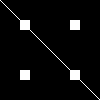
\includegraphics[width = 0.2\textwidth]{figures/newtoy/trueConn}
    \label{fig:1a} } \subfigure[]{
    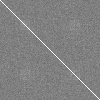
\includegraphics[width =
0.2\textwidth]{figures/newtoy/corrNoSmooth}
    \label{fig:1b} } \subfigure[]{
    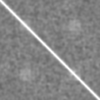
\includegraphics[width =
0.2\textwidth]{figures/newtoy/SampleCorr}
    \label{fig:1c} }\\ \subfigure[]{
    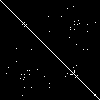
\includegraphics[width =
0.2\textwidth]{figures/newtoy/threholdCorrRaw}
    \label{fig:1d} } \subfigure[]{
    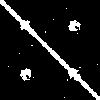
\includegraphics[width =
0.2\textwidth]{figures/newtoy/threholdCorrSmoothed}
    \label{fig:1e} } \subfigure[]{
    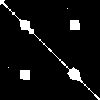
\includegraphics[width =
0.2\textwidth]{figures/newtoy/newpost_sym2}
  \label{fig:1f} }
  \caption[Test on synthetic data.]{Test of synthetic data, showing
the (a) ground-truth connectivity, (b) correlation of original, noisy
data, (c) correlation of Gaussian-smoothed data, (d) connectivity
based on noisy correlations, (e) connectivity based on smoothed data,
(f) connectivity computed using proposed MRF model.}
  \label{fig:1}
\end{figure}


% In fig. \ref{fig:1}, direct thresholding of correlation map
% (\ref{fig:1c}) or standard Gaussian mixture model (\ref{fig:1d}) does
% not use pixels' spatial context information, hence can not give a
% spatial coherent connectivity region. By using MRF in prior
% distribution, our method in fig. \ref{fig:1e} is able to get a
% clustered region while removing other scattered false positive points.

\noindent {\bf Resting-State fMRI.} Next we tested our method on real data from
healthy control subjects in a resting-state fMRI study. BOLD EPI images (TR= 2.0
s, TE = 28 ms, GRAPPA acceleration factor = 2, 40 slices at 3 mm slice
thickness, 64 x 64 matrix, 240 volumes) were acquired on a Siemens 3 Tesla Trio
scanner with 12-channel head coil during the resting state, eyes open. The data
was motion corrected by SPM software and registered to a T2 structural image. We
used a gray matter mask from an SPM tissue segmentation so that only gray matter
voxels are counted in the connectivity analysis. We do \emph{not} spatially
smooth the data, in order to see the benefit of replacing spatial smoothing with
our MRF method. Before computing the correlations, the time series at all voxels
are linearly detrended by least squares regression.

Fig.~\ref{fig:3} compares the real data results using no spatial regularization,
Gaussian smoothing, and the proposed MRF model. Though the posterior
connectivity of the MRF is computed between every pair of voxels within a slice,
for visualization purposes, only the posterior of the connectivity between one
voxel and the slice is shown. We chose to visualize the connectivity to a voxel
in the posterior cingulate cortex (PCC) because this is known to be involved in
the Default Mode Network~\cite{raichle2001}, with connections to the medial
prefrontal cortex (MPFC). The results show that Gaussian smoothing is able to
remove noise, but is unable to find a clear connection between the PCC and the
MPFC. Our proposed MRF model (rightmost plot) is able to remove spurious
connections, and also clearly shows a connection to the MPFC.

To show the strongest connections found by each method,
Fig.~\ref{fig:2} shows the thresholded connectivity maps overlaid on T2
structural image. Images in the first two columns are thresholded such that the
top $5\%$ voxel correlations are shown. For the MRF in the third column, the MAP
estimate is shown.

\begin{figure}[bth]
  \centering 
  \subfigure[]{
    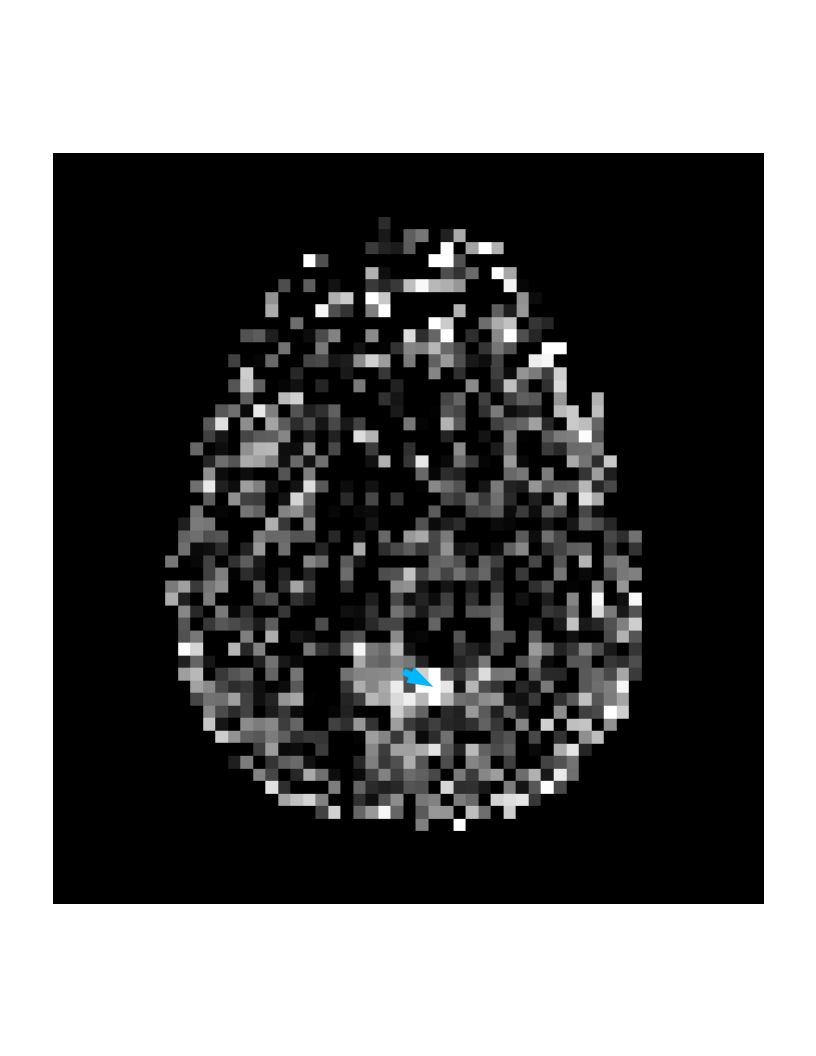
\includegraphics[width = 0.2\textwidth]{figures/no_overlay/R1_corr_nosmooth}
    \label{fig:3a}
  }
  \subfigure[]{
    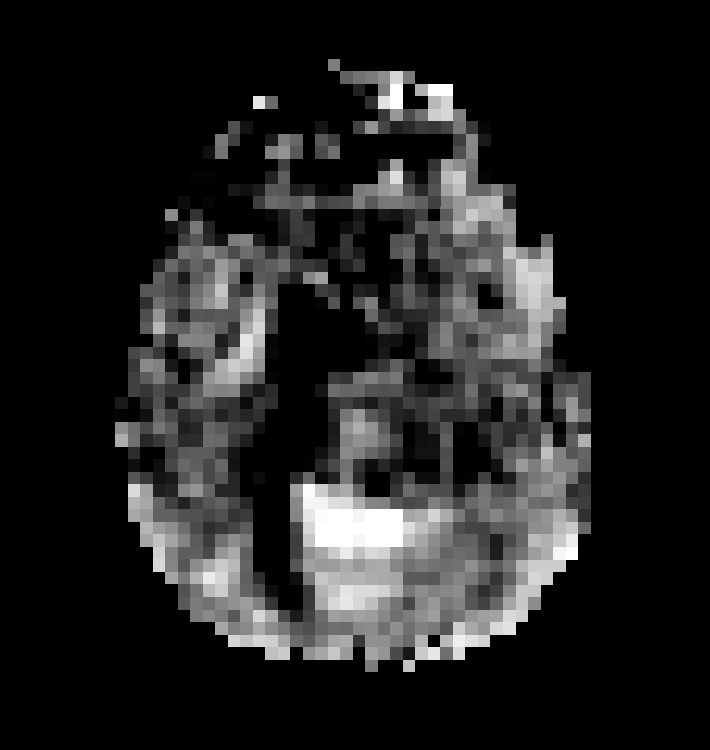
\includegraphics[width = 0.2\textwidth]{figures/no_overlay/R1_corr_smooth}
    \label{fig:3b}
  }
  \subfigure[]{
    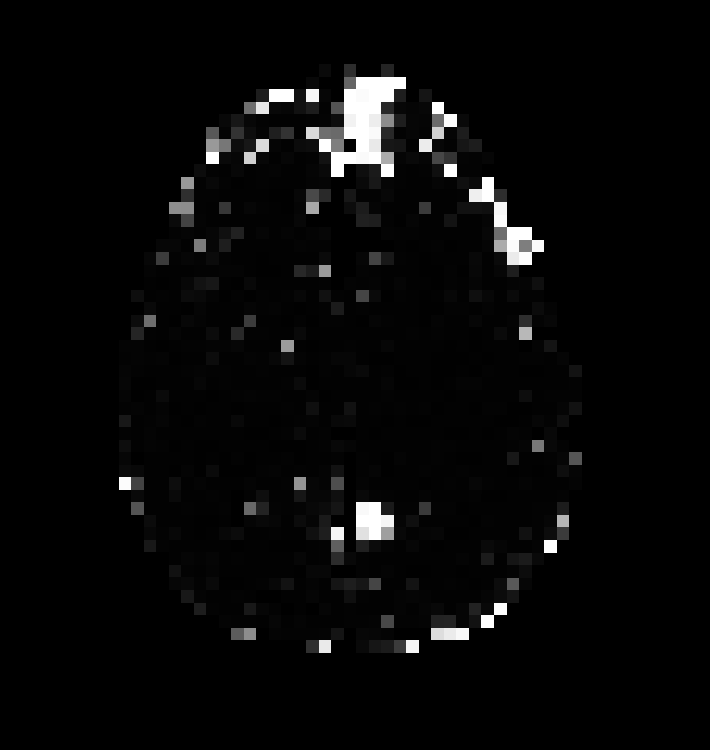
\includegraphics[width = 0.2\textwidth]{figures/no_overlay/R1_mrf}
    \label{fig:3c}
  }\\
  \subfigure[]{
    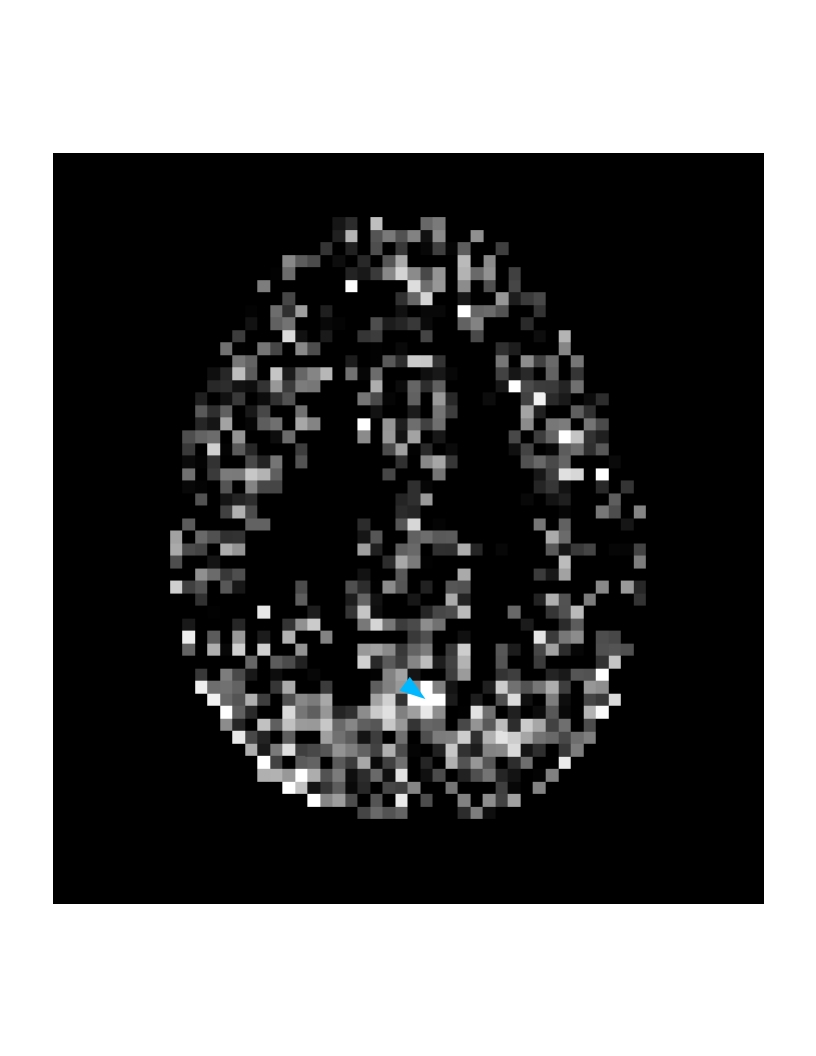
\includegraphics[width = 0.2\textwidth]{figures/no_overlay/R2_corr_nosmooth}
    \label{fig:3d}
  }
  \subfigure[]{
    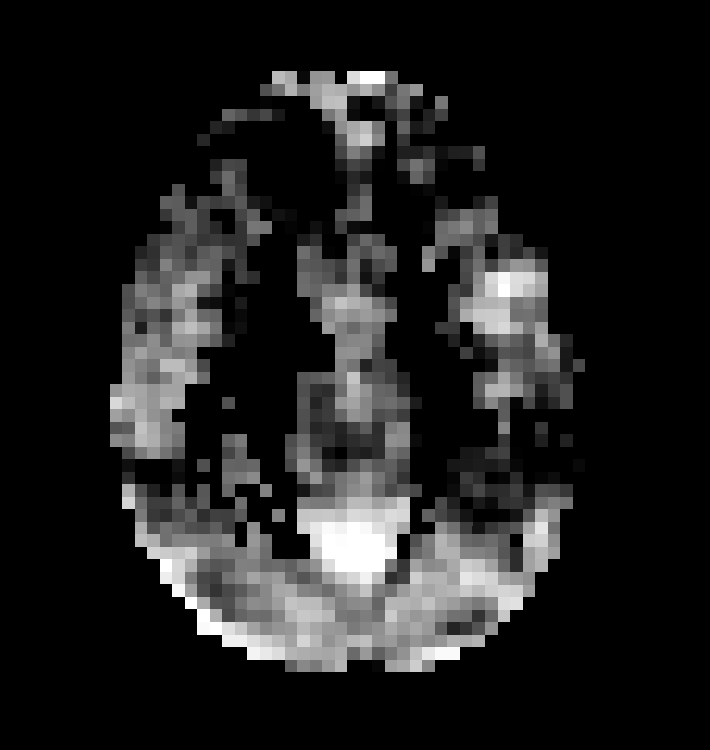
\includegraphics[width = 0.2\textwidth]{figures/no_overlay/R2_corr_smooth}
    \label{fig:3e}
  }
  \subfigure[]{
    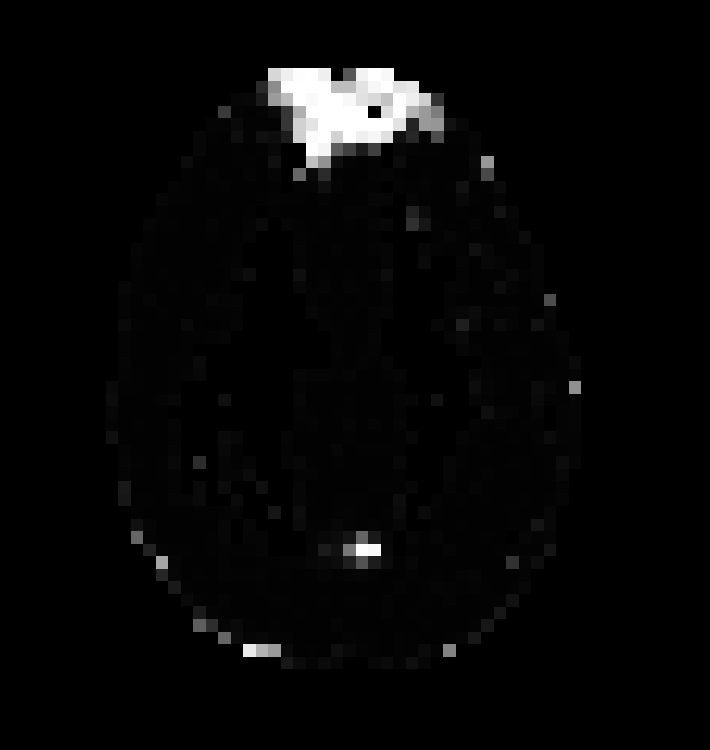
\includegraphics[width = 0.2\textwidth]{figures/no_overlay/R2_mrf}
    \label{fig:3f}
  }

  \caption[]{Correlation map and Posterior Connectivity map between
    seed voxel and slice containing the seed. First row is subject
    1. (a) the correlation map computed from data without spatial
    smoothing. (b) correlation map of data after smoothing. (c)
    Posterior probability computed from MRF. Second row (d,e,f) is
    subject 2 with same test.}
  \label{fig:3}
\end{figure}
 
\begin{figure}[htb]
  \centering 
  \subfigure[]{
    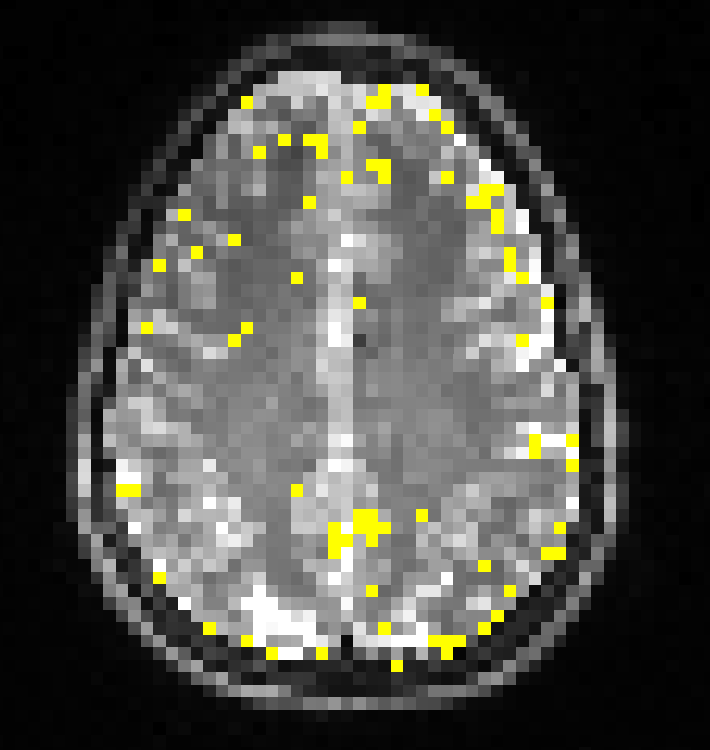
\includegraphics[width = 0.2\textwidth]{figures/thresholding_correlationMap/R1_at_gold.png}
    \label{fig:2a}
  }
  \subfigure[]{
    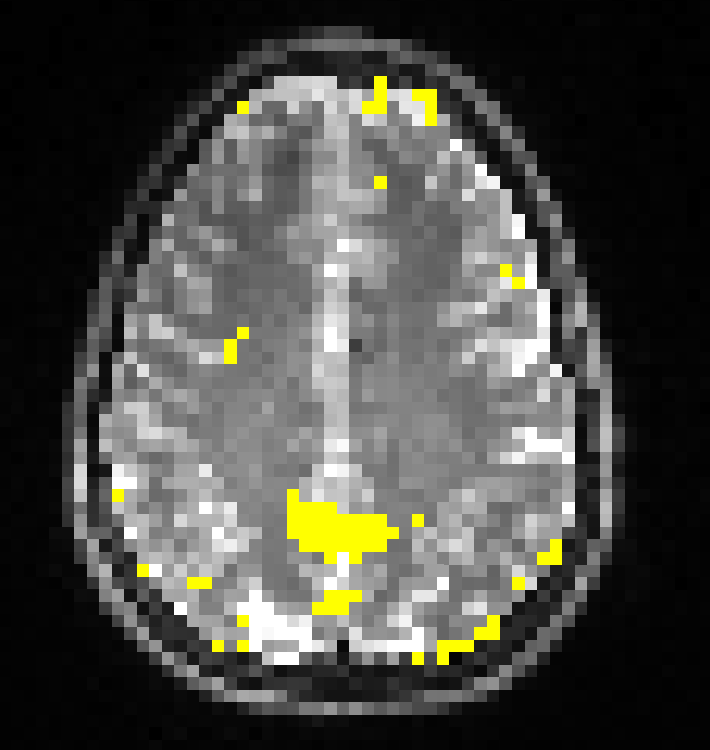
\includegraphics[width = 0.2\textwidth]{figures/threshold_smthed_corrMap/R1_at_gold.png}
    \label{fig:2b}
  }
  \subfigure[]{
    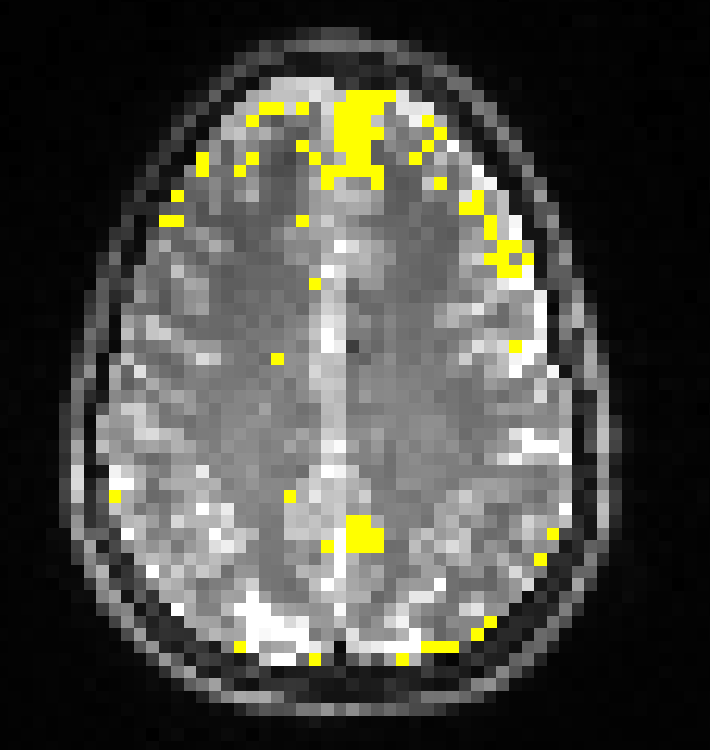
\includegraphics[width = 0.2\textwidth]{figures/mrf/R1_mrf_at_05.png}
    \label{fig:2c}
  }\\
  \subfigure[]{
    \includegraphics[width = 0.2\textwidth]{figures/thresholding_correlationMap/R2_at_gold.png}
    \label{fig:2d}
  }
  \subfigure[]{
    \includegraphics[width = 0.2\textwidth]{figures/threshold_smthed_corrMap/R2_at_gold.png}
    \label{fig:2e}
  }
  \subfigure[]{
    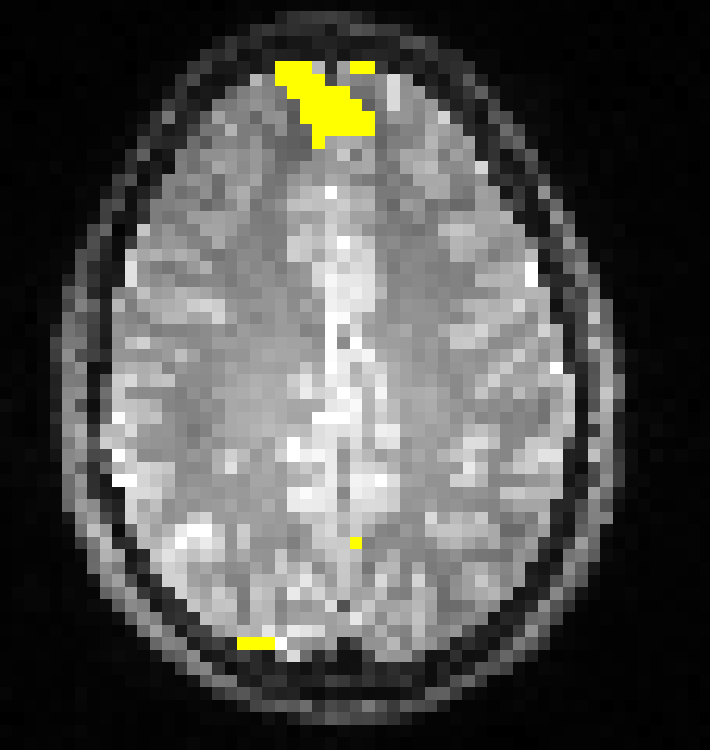
\includegraphics[width = 0.2\textwidth]{figures/mrf/R2_mrf_at_05}
    \label{fig:2f}
  }

  \caption[]{Thresholded correlation map and Posterior Connectivity
    map between seed voxel and slice, overlaid to T2 image.  First row
    is subject 1. (a) the correlation map computed from data without
    spatial smoothing. (b) After smoothing. (c) Posterior probability
    by MRF. Second row (d,e,f) is subject 2 with same test. }
  \label{fig:2}
\end{figure}
\section{Conclusion}
We propose a Markov random field and Bayesian framework for spatially regularizing functional connectivity. Future work may include running this pairwise connectivity analysis on 3D whole brain. Another interesting direction is applying the method to multiple sessions and subjects. 

\section{Acknowledgments}
This work was funded in part by NIH Grant R01 DA020269 (Yurgelun-Todd).

\bibliographystyle{splncs} 
\bibliography{newreference}
\end{document}
   
